\section{Data Preparation}

Mit den Erkenntnissen aus der vorherigen Phase beginnt nun die Aufbereitung der Daten. Jede Komponente bzw. jedes System hat im Project RA Application Conditions einen Ordner \glqq 10\char95 Project
Answers\grqq{}. Nutzt ein Projekt nun beispielsweise das Achszähler-System AzS350U und hat die Anwendungsregeln des Systems bewertet, dann müssen diese bewerteten Anwendungsregeln in ein neues Modul 
in dem \glqq 10\char95 Project Answers\grqq{} Ordner des Achszähler-Systems geschrieben werden \cite[S.21]{q2}. Mit den Modulen, die die bewerteten Anwendungsregeln der einzelnen Komponenten und Systeme 
beinhalten, kann dann das KI-System angelernt werden. 

Um das zu erreichen, müssen zunächst die 115 Module genauer untersucht werden. Dabei muss geprüft werden, ob diese Module die Anwendungsregeln so bewertet haben, wie es das Process Manual vorgibt.
Dafür muss die Iteration aus \ref*{lst:searchInLinks} erweitert werden. Es muss zusätzlich geprüft werden, ob das Modul die Attribute REQ Status bzw. REQ Progress besitzt und ob diese auch 
ausgefüllt sind. 

\begin{lstlisting}[caption={Suche nach bewerteten Anwendungsregeln},captionpos=b, label = lst:searchARSolutions]                                                       
if(hasAttribute("REQ Status", mod) 
&& hasAttribute("REQ Statement", mod)){  
    szProgress = o."REQ Status""";
    szStatement = o."REQ Statement";
    if(length(szProgress)>1 && length(szStatement)>1){ 
        put(slResults, fullName mCheck, fullName mCheck)
    }
}else if (hasAttribute("REQ Progress", mod) 
&& hasAttribute("REQ Statement", mod)){
    szProgress = o."REQ Progress""";
    szStatement = o."REQ Statement";
    if(length(szProgress)>1 && length(szStatement)>1){ 
        put(slResults, fullName mCheck, fullName mCheck)
        // ...
\end{lstlisting}

Übrig bleiben danach 41 Module aus 34 Projekten, welche nicht nur die Anwendungsregeln importiert, sondern auch nach den Vorgaben des Process Manuals bewertet haben. Als Zwischenschritt wurde daraufhin
für jedes Projekt ein Modul in meiner Sandbox erstellt. In diesem Modul wurden dann alle bewerteten Anwendungsregeln reingeschrieben. Dabei musste darauf geachtet werden, dass auschließlich die
Anwendungsregeln in das Modul geschrieben wurden und keine Überschriften oder Ähnliches. Zudem durften nur die relevanten Attribute in dem neuen Modul stehen. Alle weiteren Attribute dürfen nicht
hinzugefügt werden, da diese für das Bewerten von Anwendungsregeln irrelevant sind und die Module und somit den schlussendlichen Datensatz, welcher zum Trainieren des KI-Systems verwendet werden soll,
unnötig groß machen würden. Zudem muss, wie in Kapitel \ref*{chap:DataUnderstanding} beschrieben, überprüft werden, ob sich die Anwendungsregel unter dem Punkt 
\glqq Old Version Objects, to be reviewed and deleted: \grqq{} befindet. Dafür muss über alle Väter eines Objekts iteriert werden und geprüft werden, ob die Überschrift eines Objekts 
\glqq Old Version Objects, to be reviewed and deleted: \grqq{} ist. Der Quellcode \ref*{lst:checkOld} zeigt eine Möglichkeit, bei der eine Boolean-Variable auf true gesetzt wird, falls ein Objekt
veraltet ist. Diese Objekte werden dann nicht in das neue Modul geschrieben.

\begin{lstlisting}[caption={Prüfen, ob Objekt veraltet ist}, captionpos=b, label = lst:checkOld] 
for obj in entire mod do{ 
    oParent = parent(obj)
    bOldVersion = false;
    while (oParent != null){
        if (oParent."Object Heading""" ==  "Old Version Objects, to be reviewed and deleted:"){
            bOldVersion = true;
        }
        oParent = parent(oParent)
    }
\end{lstlisting}

Abbildung \ref*{fig:SolutionsModul} zeigt, wie ein Modul für ein Projekt dann aussieht. Erkennbar ist, dass dort lediglich die relevanten Attribute gespeichert werden. Zudem wird ein Out-Link auf die
Anwendungsregel unter RA Application Conditions gesetzt, damit nachverfolgt werden kann, von wo die Anwendungsregel ursprünglich stammt. Des Weiteren besteht der Name des Moduls aus dem Namen
des Projekt sowie der Endung \char95 Solutions. Dadurch wird sichergestellt, dass die Information darüber, von welchem Projekt die bewertete Anwendungsregel stammt, erhalten bleibt.

\begin{figure}[H]
    \centering
    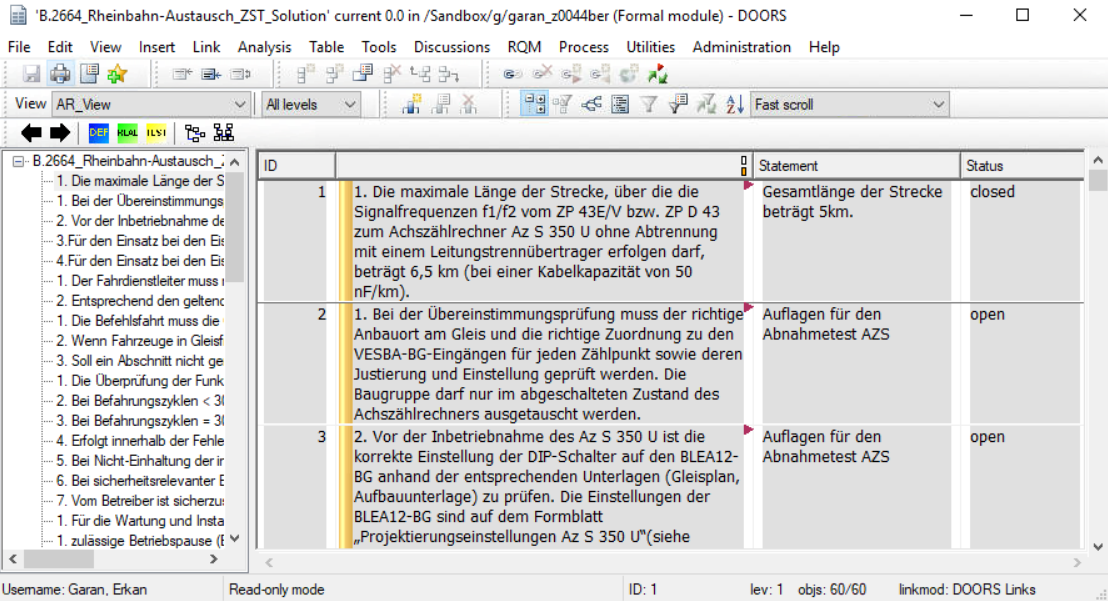
\includegraphics[width = \textwidth]{abbildungen/Solutions.PNG}
    \caption{Modul eines Projekts}
    \label{fig:SolutionsModul}
\end{figure}

Im nächsten Schritt müssen diese Solution-Module der einzelnen Projekte noch weiter aufgeteilt werden. Durch den Out-Link jedes Objekts kann geprüft werden, von welcher Komponente oder System die
Anwendungsregel stammt. Daraufhin müssen alle Anwendungsregeln eines Projekts, die von der selben Komponente oder vom selben System stammen in ein eigenes Modul ausgegliedert werden, welches dann
in den Project Answers Ordner der Komponente oder des Systems verschoben wird. Dafür wird über alle Objekte im Solution-Modul eines Projekts iteriert. Jedes Objekt wird dann 
in ein Modul kopiert, dessen Name sich aus dem Projektnamen sowie des Namens der Komponente oder des Systems. Letzterer Name wird dabei aus dem Out-Link übernommen. Diese Module müssen dann 
zum Schluss in den jeweilegen Project Answers Ordner verschoben werden.

\begin{figure}[H]
    \centering
    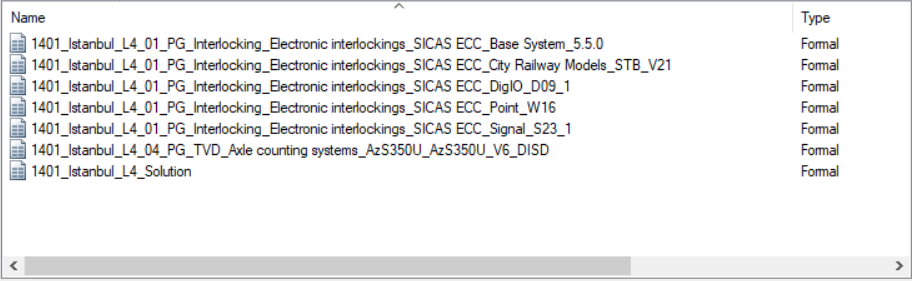
\includegraphics[width = \textwidth]{abbildungen/Aufgeteilte Module.PNG}
    \caption{Aufgeteiltes Solution-Modul}
    \label{fig:AufgeteilteModule}
\end{figure}

Bevor die Module verschoben werden, wird vorher der Datensatz zum Anlernen des KI-Systems im .csv-Format erstellt. Dieser
Schritt wird eingeschoben, da zu diesem Zeitpunkt die Module zentral in meiner Sandbox liegen und es somit einfacher ist über all diese Module zu iterieren. Dabei wird wieder über jedes Objekt
von jedem Modul iteriert und dabei der Objekt Text, der Status sowie das Statement in eine Variable vom Typ String geschrieben. Bei dem Objekt Text und bei dem Statement müssen alle Kommata entfernt
werden, da diese sonst zu Problemen bei der .csv-Datei führen würden. Dafür wurde eine Methode erstellt, die alle Kommata eines Textes entfernt. Anschließend werden die drei Variablen an eine
String-Variable konkateniert, welche am Ende jedes Moduls in die .csv-Datei geschrieben wird. Für das Schreiben in diese Datei musste ebenfalls eine weitere Methode geschrieben werden. 
Der String, welcher in die Datei geschrieben wird, hat dann die Form:

\begin{quotation}
    \noindent
    \dq Anwendungsregel\dq,\dq Status\dq,\dq Statement\dq \linebreak
    \dq Anwendungsregel\dq,\dq Status\dq,\dq Statement\dq \linebreak
    ...
\end{quotation}

\begin{lstlisting}[caption={Daten in eine .csv-Datei schreiben}, captionpos=b, label = lst:writeCSV]
// ...
m = read(fullName(it), false)
for o in entire m do{
    szText = cleanText(o."Object Text""")
    szStatus = o."Status"
    szStatment = cleanText(o."Statement""")
    szData = szData "\"" szText "\",\""szStatus"\",\""szStatment"\"\n"
}
writeCSV(szData)
// ...
\end{lstlisting}

Nun wurde eine .csv-Datei mit dem finalen Datensatz erstellt, welcher später für das Anlernen eines unterstützenden KI-Systems zum Bewerten von Anwendungsregeln verwendet werden kann.
Dieser Datensatz umfasst dabei 195.518 bewertete Anwendungsregeln aus Projekten der Siemens Mobility GmbH. Zum Schluss können nun alle Module in ihre entsprechenden Project Answers Ordner 
verschoben werden. 
